\chapter{Simulation Physics}
\label{ch:SimPhys}
This chapter outlines the physical principles and relevant formulas for the simulation of rigid and deformable bodies.
It is essential to understand the modeling of rigid and deformable bodies in order to investigate possibilities to interact with the bodies for collision handling.

We first give a brief overview over the simulation of single bodies and afterwards describe the simulation of rigid and deformable bodies in detail.
Subsequently, we discuss how to interact with the bodies for collision handling and outline the integration scheme.

\section{Single Body Dynamics}
\label{sec:MultiBodyDynamics}
The laws of physics provide an exact and comprehensive description of the physical behavior of bodies. Since an exact and comprehensive representation of these laws in multi-body-simulations is not feasible, due to the complexity of these descriptions approximations and adaptations with regard to the intended use are necessary.

In this work, we simulate different types of bodies. We simulate rigid and deformable bodies, additionally we use geometry that does not move, which we call static bodies.
Non-static bodies change their motion due to the effects of forces, described by Newton's second law of motion. The way how these changes take place depends on whether the body is deformable or rigid.  In contrast to rigid bodies, deformable bodies also change their shape in response to applied forces \cite{BENDER2007}.

\subsection{Rigid Body Dynamics}
\label{sec:RigidBodyDynamics}
A rigid body is an idealized model of a solid body in which deformation is neglected.
Thereby, it can by described by only six degrees of freedom: translations along three axes of space and rotations around these three axes \cite{BENDER2007}.

The translation is determined by the body's mass $m$, position $\mathbf s(t)$ and velocity $\mathbf v(t)$. The rotation is determined by the body's inertia tensor $\mathbf J$, the rotation matrix $\mathbf R(t)$ and the angular velocity $\boldsymbol{\omega}(t)$.  The translational movement is influenced by the exterior forces $\mathbf f_{ext}$ and can be expressed by a system of linear first order differential equations
\begin{align}
    \dot{\mathbf{v}}&=\frac{\mathbf f_{ext}}{m}\\
     \dot{\mathbf{x}}&=\mathbf v 
\end{align}
For constant forces, as it is the case within a simulation time step $\Delta t$, the system can be solved analytically and no numerical integration is necessary. The velocity can be computed by
\begin{equation}
      \mathbf v(t_0+\Delta t)=\mathbf v(t_0) +\int\limits_{0}^{\Delta t}\dot {\mathbf{v}}dt=\mathbf v(t_0)+\frac{1}{m} \mathbf f_{ext}\Delta t.
\end{equation}
The new position is determined by
\begin{align}      
      \mathbf x(t_0+\Delta t)&=\mathbf x(t_0)+\int\limits_{0}^{\Delta t}\dot {\mathbf{x}}dt=\mathbf x(t_0)+\int\limits_{0}^{\Delta t}\mathbf v(t_0)+\frac{1}{m}\mathbf f_{ext} t \;dt\\      
     &=\mathbf x(t_0)+\mathbf v(t_0)\Delta t + \frac{1}{2m}\mathbf f_{ext}\Delta t^2.
\end{align}
The rotational movement is influenced by the exterior torque $\boldsymbol \tau_{ext}$. The change in angular velocity can be expressed by the Euler-Equation
\begin{equation}
       	\boldsymbol {\dot{\omega}} =\mathbf J^{-1}(\boldsymbol \tau_{ext}-[\boldsymbol \omega(t)\times[\mathbf J\boldsymbol \omega(t)]]).
\end{equation}

The Euler-Equation is handled by a transformation into the local coordinate system, in which $\mathbf J$ is constant and then solved with a numerical integration method.
The change in rotation can be expressed in terms of $\mathbf R(t)$ 
\begin{equation}
\label{eq::dR_R}
		\dot{\mathbf{R}}(t)=\boldsymbol \omega^*(t) \mathbf R(t).
\end{equation}
with $\boldsymbol \omega^*(t)$ denoting the cross product matrix of $\boldsymbol \omega(t)$.

However, representing the rotation with a rotation matrix $\mathbf R$ is redundant, since nine values are used to express three degrees of freedom. Furthermore, the formulation is numerically unstable. Alternatively, the rotation can be expressed in a more stable and less redundant way with unit quaternions 
\begin{equation}
\label{eq::dR_q}
	\dot{\mathbf{q}}(t)=\frac{1}{2}\boldsymbol\omega(t)\cdot  \mathbf q(t).
\end{equation}
A unit quaternion is a normalized 4-element vector and the above used notation is the short form of $(0,\omega_x(t),\omega_y(t),\omega_z(t))\cdot \mathbf{q}(t)$ \cite{BENDER2007}. 
Thus, it is less redundant and more stable. Both equations \ref{eq::dR_R} and \ref{eq::dR_q} can be solved using numerical integration.

Furthermore, impulses can be applied to the body.
For an impulse $\mathbf I$ the relation
\begin{equation}
\label{eq::impulse}
	\mathbf I=m\mathbf v
\end{equation}
applies and similarly for a rotational impulse $\mathbf l$
\begin{equation}
\mathbf	l=\mathbf J\boldsymbol\omega.
\end{equation}

The previously presented equations apply for centered impulses and forces. If a non-centred force $\mathbf f$ is applied, the rotational torque component $\boldsymbol\tau$ computes as
\begin{equation}
\boldsymbol\tau= \mathbf d\times \mathbf f\\
\end{equation}
with the distance vector $\mathbf d$ from the center of mass to the point of application. Similarly the rotational impulse $\mathbf l$ for a non-centered impulse $\mathbf I$ computes as
\begin{equation}
\mathbf l=\mathbf d\times \mathbf I.
\end{equation}
In our framework, the rigid body dynamics are computed with the open source Bullet physics library \cite{COUMANS2006}. Nevertheless, it is important to introduce the formulas as a basis for the collision handling.

\subsection{Deformable Body Dynamics}
\label{sec:DeformaleBodyDynamics}
Deformable bodies change their shape in response to applied forces, which makes them more complex to simulate than rigid bodies. In our framework, deformable bodies are modeled with finite elements with quadratic bases for the simulation \cite{WEBER2011}. Nevertheless, as a basis for the collision handling it is sufficient to examine linear finite elements \cite{MUELLER2004}.
% providing high stability and plausible deformation.\\
The method of finite elements for deformable bodies is based on the Lagrange equation for the dynamic behavior of an object. The Lagrange equation can be formulated for the position $\mathbf x(t)$ as
\begin{equation}
\label{eq::defbodies_lag}
\mathbf {M}\ddot{\mathbf{x}}+\mathbf{C}\dot{ \mathbf{x}}+\mathbf{K(x-x_0)=f_{ext}},
\end{equation}
with the first and second order derivatives of the position vector $\mathbf x$, $\dot {\mathbf x}$ and $\ddot {\mathbf x}$, the mass matrix $\mathbf M$, the damping matrix $\mathbf C$, the stiffness matrix $\mathbf K$ and the external forces $\mathbf f_{ext}$. For a system with $n$ vertices, equation \ref{eq::defbodies_lag} gives a coupled system of $3n$ linear ordinary differential equations.
To compute the stiffness matrix $\mathbf K$, we need to understand how the stiffness matrix $\mathbf K_e$ for a single tetrahedron is computed.

For a continuous object, the deformation of a point $\mathbf y \in \mathbb R^3$ is defined by a vector field $\mathbf u(\mathbf y)$ as
\begin{equation}
\mathbf {x(y)=y+u(y)},
\end{equation}
with the deformed position $\mathbf {x(y)}$. With a linear finite element approach, the deformation is linearly interpolated between the four vertices of the tetrahedron as
\begin{equation}
\mathbf {u(y)}=\mathbf H_e(\mathbf y) \hat {\mathbf u},
\end{equation}
with the shape function $\mathbf H_e(\mathbf y)$ and the displacement vector $\hat {\mathbf u}$, containing the displacement vectors of the four tetrahedron vertices.
Using Cauchy's linear strain tensor \cite{COOK1994} the strain $\boldsymbol\varepsilon$ is
\begin{equation}
\boldsymbol \varepsilon=\frac{1}{2} (\frac{\partial \mathbf u}{\partial \mathbf y}+\frac{\partial \mathbf u}{\partial \mathbf y}^T)=\mathbf B_e  \hat{\mathbf u},
\end{equation}
with the constant matrix $\mathbf B_e$ containing derivations of $\mathbf H_e(\mathbf y)$. Applying Hooke's law, the stress $\boldsymbol \sigma$ within an element is
\begin{equation}
\boldsymbol \sigma=\mathbf E \boldsymbol\varepsilon=\mathbf E \mathbf B_e \hat{\mathbf u},
\end{equation}
with the constant matrix $\mathbf E$ describing the material's elasticity. For isotropic materials, $\mathbf E$ only depends on two scalars, namely the Young's modulus and the Poisson's ratio.

Finally, the stiffness matrix $\mathbf K_e$ for one tetrahedron results in
\begin{equation}
\mathbf f_e=\mathbf V_e \mathbf B_e^T \mathbf E \mathbf B_e \hat{\mathbf u}=\mathbf K_e \hat{\mathbf u},
\end{equation}
with the tetrahedron's volume $\mathbf V_e$ and the elastic forces $\mathbf f_e$. Assembling all matrices $\mathbf K_e$ gives the final stiffness matrix $\mathbf K$.

Now equation \ref{eq::defbodies_lag} can be solved with time integration. We use implicit Euler integration, since it provides unconditional stability \cite{WEBER2011}, what is a crucial property in interactive systems. %With the implicit Euler the time discretization yields a linear system
%\begin{gather}
%  (\mathbf{M}+\Delta t \mathbf{D}+ \Delta t^2 \mathbf{K})\Delta\mathbf{v}= - \Delta t (\mathbf{K}\mathbf{x}+\mathbf{f_0-f_{ext}}+\Delta \mathbf{Kv+Dv})\\
%   \Delta \mathbf{x}
%    =\Delta (\mathbf v +\Delta \mathbf{v}),
%\end{gather}
%which can be solved with the method of conjugated gradients.
\section{Interacting with Rigid and Deformable Bodies}
\label{sec:InteractingRigDef}
To handle collisions we need to act upon the bodies' dynamics in order to counteract the penetrations.

As we have seen in the previous two sections, the movement of rigid and deformable bodies can be influenced by applying external forces, which directly apply on the acceleration. Furthermore, it is possible to change the velocities by applying impulses or to modify the positions directly.

In the simulation we split the integration in two steps. In the first step, the so called velocity step, we compute the new velocities according to the bodies' interior dynamics and the external forces as presented in section \ref{sec:RigidBodyDynamics} and section \ref{sec:DeformaleBodyDynamics}. Afterwards, in the second step, the so called position step, the new positions are computed based on the new velocities. Therefore, it is reasonable to apply additional forces before the velocity step, to modify velocities by applying impulses between the velocity and position step and to modify positions after the position step. 

In this work, we apply impulses as suggested by Tang et al. \cite{TANG2012}, since the result of the CPF algorithm are impulses.

Applying impulses on rigid bodies is straightforward, see section \ref{sec:RigidBodyDynamics}.
For deformable bodies applying impulses is more complex. In contrast to rigid bodies, deformable bodies do not have one global velocity, but each vertex has its own velocity and its associated mass. Therefore, we can apply impulses at the vertices, analogously to the formula for centered impulses for rigid bodies, see equation \ref{eq::impulse}.
If the point of application is not a vertex it is necessary to determine the triangle including the point of application. Thereby, the barycentric weights can be computed and the impulse is divided on the triangle vertices according to the barycentric weights \cite{TANG2012}.




%These approaches equate to modify the position, its first derivation the velocity or its second derivation the acceleration.
%By modifying a high derivation we yield a consistent result, since if we modify the acceleration with forces, velocity and position are updated accordingly in the integration scheme and the mass is included. Whereas, if we modify the position there is not necessarily an effect on the velocity.
%However, modifying the position provides a higher level of control than modifying the forces.


\section{Time Integration}
\label{sec:TimeIntegration}
To step the simulation forward in time, we separate the bodies' internal dynamics from the collision processing algorithm similarly to Bridson et al. \cite{BRIDSON2002}.
The collisions are handled in a predictor-corrector fashion (see figure \ref{fig:pre_corr}). We first predict the velocities (1) and positions at the end of the time step, then we use the predicted information to check for collisions (2). If collisions are detected, we apply the collision resolution algorithm to compute the repulsion impulses and corrected velocities (3) and use the corrected velocities to compute the final positions (4).
\begin{figure}[h] 
  \centering
     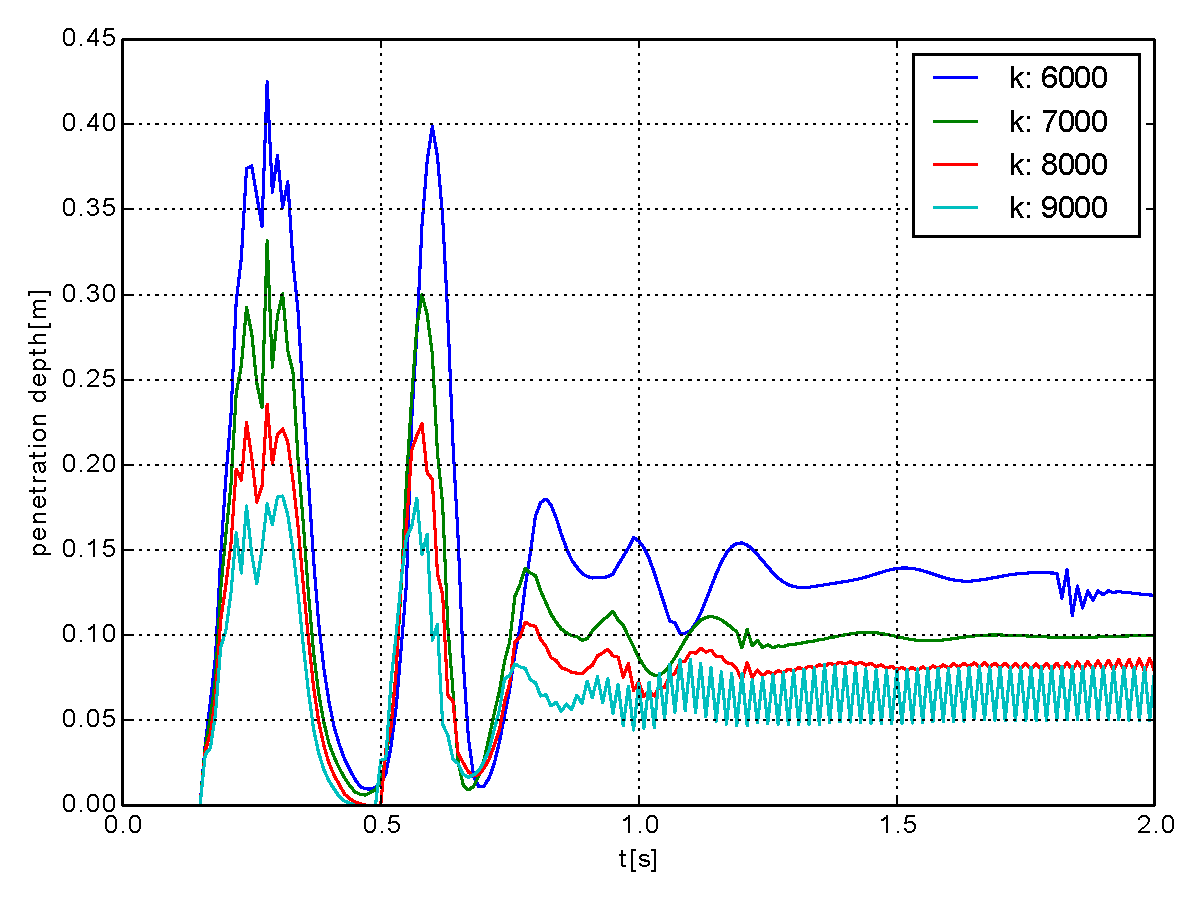
\includegraphics[width=0.9\textwidth]{pics/pdf/pre_corr.pdf}
  \caption[Predictor-Corrector scheme]{Illustration of the predictor-corrector scheme showing a particle colliding with a plane. 1) Prediction of the new velocity  2) Check for collisions along the new trajectory
  3) Applying correction impulses yields the final velocity
  4) Position update}
  \label{fig:pre_corr}
\end{figure}

In contrast to Bridson we do not check for proximity  since we do not differ between collision and contact and apply friction together with the repulsion impulses. So the integration scheme can be expressed as
\begin{enumerate}
\item
Advance simulation by one time step $\Delta t$ and set: $t^{n+1}=t^{n}+\Delta t$
\item
Predict new candidate velocities $\mathbf v^{n+1}_p$ according to external forces and bodies' interior dynamics 
\item Check linear trajectories for collisions between $t^n $ and $t^{n+1}$ using the position from the previous step $\mathbf x^n$ and $\mathbf v^{n+1}_p$
\item Repeat until no new collisions appear, maximum 5 iterations
	\begin{enumerate}[label*=\arabic*.]
	\item Compute repulsion and friction impulses for unhandled collisions
	\item Update $\mathbf v^{n+1}_p$ with the repulsion and friction impulses
	\item Check linear trajectories for collisions between $t^n $ and $t^{n+1}$ using the position from the previous step $\mathbf x^n$ and $\mathbf v^{n+1}_p$
	\end{enumerate}
	
\item Update velocity $\mathbf v^{n+1}=\mathbf v^{n+1}_p$
\item Update positions $\mathbf x^{n+1}=\mathbf x^n+ \Delta t \mathbf v^{n+1}$
\item Check for collision resolution and for redefinition
\item Rendering
\end{enumerate}
% Sunil Hadap, Dave Eberle, Pascal Volino, Ming C. Lin,
%Stephane Redon, and Christer Ericson. Collision detection and
%proximity queries proposed handling in chronological order
